\documentclass[12pt,landscape,a4paper]{article}

%%%%%% Cheatsheet Template %%%%%%%%%%%%%%
%Authors: Simon Vilmin, Johann Laconte
%%%%%%%%%%%%%%%%%%%%%%%%%%%%%%%%%%%%%%%%%

\usepackage[dvipsnames]{xcolor}
\usepackage[utf8]{inputenc}
\usepackage[english]{babel}
\usepackage[T1]{fontenc}
\usepackage{multicol}
\usepackage[top=5mm,bottom=8mm,left=8mm,right=5mm]{geometry}
\usepackage{pdfpages}
\usepackage{amsmath}
%\usepackage{amsthm}
\usepackage{array}
\usepackage{wrapfig}
\usepackage[compact]{titlesec}  % compact : no space around titles
\newcolumntype{L}[1]{>{\raggedright\let\newline\\\arraybackslash\hspace{0pt}}m{#1}}
\newcolumntype{C}[1]{>{\centering\let\newline\\\arraybackslash\hspace{0pt}}m{#1}}
\newcolumntype{R}[1]{>{\raggedleft\let\newline\\\arraybackslash\hspace{0pt}}m{#1}}

%Load colors
%from https://flatuicolors.com/
\definecolor{blueSection}{cmyk}{1,.72,0,.38}
\definecolor{blueMath}{rgb}{.17,.22,.34}
\definecolor{alizarine}{RGB}{231, 76, 60}
\definecolor{silver}{RGB}{189, 195, 199}
\definecolor{pomegranate}{RGB}{192, 57, 43}
\definecolor{midnight}{RGB}{44, 62, 80}
\definecolor{belize}{RGB}{0, 103, 176}
\definecolor{cyan}{RGB}{0, 188, 212}
\definecolor{teal}{RGB}{0, 150, 136}
\definecolor{greal}{RGB}{0, 130, 116}
\definecolor{sang}{RGB}{183, 28, 12}
\definecolor{emerald}{RGB}{0, 140, 49}
\definecolor{sunflower}{RGB}{241, 196, 15}
\definecolor{amethyst}{RGB}{155, 89, 182}
\definecolor{turquoise}{RGB}{0, 139, 128}
\definecolor{asbestos}{RGB}{127, 140, 141}
\definecolor{clouds}{RGB}{236, 240, 241}
\definecolor{lynch}{HTML}{3E4651}
\definecolor{clearsky}{HTML}{83D6DE}
\definecolor{greensea}{RGB}{22, 140, 113}
\definecolor{grass}{HTML}{97CE68}
\definecolor{peter}{RGB}{92, 192, 255}
\definecolor{lightmethyst}{RGB}{175, 109, 202}
\definecolor{pumpkin}{RGB}{211, 84, 0}
\definecolor{desire}{RGB}{181, 52, 113}
\definecolor{orangeville}{RGB}{225, 112, 85}
\definecolor{wetAsphalt}{HTML}{34495E}
\definecolor{americanRiver}{RGB}{99, 110, 114}

%%%%%%%%%%%%%%%%%%%FONTS%%%%%%%%%%%%%%%%%%%%%%%%%%%
    %change font here if needed
    \usepackage[nosf]{kpfonts}
	\usepackage[t1]{sourcesanspro}

    \DeclareMathSizes{11}{12}{9}{9}
    
%%%%%%%%%%%%%%%%%%%COLORS%%%%%%%%%%%%%%%%%%%%%%%%%%
    %set colors for math environments
    \everymath\expandafter{\the\everymath \color{blueMath}}
    \everydisplay\expandafter{\the\everydisplay \color{blueMath}}
    
    %set colors for titles
    \newcommand{\sectionColor}{pumpkin}
    \newcommand{\subsectionColor}{americanRiver}
    \newcommand{\numberingColor}{asbestos}
%%%%%%%%%%%%%%%%%%%%%%%%%%%%%%%%%%%%%%%%%%%%%%%%%%%

%compress text
\renewcommand{\baselinestretch}{.9}

%define header
\newcommand{\header}{
    \begin{tabular}{L{.2\linewidth} C{.5\linewidth} R{.25\linewidth}}
    J. Laconte &% author
    {\huge Lie Algebra for Robotics } &% Title
    
\includegraphics[height=2.5em]{cheatsheet_template/norlab_logo_acronym_dark.pdf} %logo
    \end{tabular}
    
    \noindent\textcolor{americanRiver}{\rule{\textwidth}{2pt}}
}

\pagestyle{empty}
 
%Define title styles (package titlesec) 
\titleformat{\section}[hang]
    {\bfseries}
    {\hspace{-1em} \textcolor{\numberingColor}{\thesection}\hspace{0.1em}\textcolor{asbestos}{\textbar}} % before title
    {0.2em}  % hspace
    {\bfseries\sffamily\color{pumpkin}} % title
    
\titleformat{\subsection}[hang] %subsection
    {\small\bfseries}
    {\hspace{-.6em} \textcolor{\numberingColor}{\thesubsection}\hspace{0.1em}}
    {0.2em}
    {\small\bfseries\sffamily\color{\subsectionColor}}
    
\titleformat{name=\subsection, numberless}[hang] %subsection*
    {\small\bfseries}
    {\textcolor{\numberingColor}{\textbar}}
    {0.2em}
    {\small\bfseries\sffamily\color{\subsectionColor}}

%remove some vertical space around equations and (sub)sections titles 
\AtBeginDocument{%
	\setlength\abovedisplayskip{.5em}
	\setlength\belowdisplayskip{.2em}
	\setlength\abovedisplayshortskip{-.5em}
	\setlength\belowdisplayshortskip{0em}}

%remove indent 
\setlength{\parindent}{0pt}

% %new environment for figures in multicol
\newenvironment{Figure}
  {\par\medskip\noindent\minipage{\linewidth}}
  {\endminipage\par\medskip}

%add some spacing beween the columns
\setlength\columnsep{1.5em}

\usepackage{mathtools}
\usepackage[all]{xy}
\usepackage{bm}

\newcommand{\GL}{\mathrm{GL}}
\newcommand{\SO}{\mathrm{\mathbf{SO}}}
\newcommand{\SE}{\mathrm{\mathbf{SE}}}
\newcommand{\so}{\mathfrak{so}}
\newcommand{\se}{\mathfrak{se}}

\newcommand{\R}{\mathbb{R}}
\newcommand{\I}{\bm{\mathrm{I}}}
\newcommand{\vzero}{\bm{0}}
\newcommand{\C}{\bm{C}}
\newcommand{\T}{\bm{T}}
\newcommand{\aT}{\bm{\mathcal{T}}}
\newcommand{\J}{\bm{J}}
\newcommand{\Jc}{\bm{\mathcal{J}}}
\newcommand{\bepsilon}{\bm{\epsilon}}
\newcommand{\bvarepsilon}{\bm{\varepsilon}}
\newcommand{\bphi}{\bm{\phi}}
\newcommand{\bPhi}{\bm{\Phi}}
\newcommand{\bxi}{\bm{\xi}}
\newcommand{\bXi}{\bm{\Xi}}

\DeclareMathOperator{\Ad}{Ad}
\DeclareMathOperator{\ad}{ad}
\DeclareMathOperator{\tr}{tr}

\begin{document}
\header
\begin{multicols*}{3}
\section{Lie Groups}
	A Lie Group is a group whose elements are organized continuously and smoothly, making it a smooth manifold.
	\subsection*{Special Orthogonal group $\SO(3)$}
		Group of 3D rotation matrix:
		$$\SO(3) = \left\{ \C \in \GL(3,\R) \,\middle|\, \det(\C)=1, \C^T\C=\I\right\}$$%
	\subsection*{Special Euclidian group $\SE(3)$}
		Group of 3D transformation matrix:
		$$\SE(3) = \left\{ %\T =%
			\begin{bmatrix}
				\C & \mathbf{r} \\
				\vzero^T & 1
			\end{bmatrix} \in \GL(4,\R)
		\,\middle|\, \C\in\SO(3), \mathbf{r}\in\mathbb{R}^3 \right\}$$

\section{Lie algebra}
	\begin{wrapfigure}[7]{r}{.5\linewidth}
		\vskip-4em
		\centering
		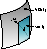
\includegraphics[width=.9\linewidth]{media/SO3.pdf}
	\end{wrapfigure}
	A Lie algebra $\mathfrak{g}$ of a Lie group $G$ is the tangent space of $G$ at the identity element.
	The tangent space is defined as the set $ \{ \gamma'(0) \}$ where $\gamma(t)\in G, \gamma(0) = \I$

	\subsection*{Special Orthogonal Group $\so(3)$}
		$$\so(3) = \left\{ \bPhi = \bphi^\wedge =%
			\begin{bmatrix}
				0 & -\phi_3 & \phi_2 \\
				\phi_3 & 0 & -\phi_1 \\
				-\phi_2 & \phi_1 & 0\\
			\end{bmatrix}
		\,|\, \bphi \in \R^3 \right\}$$

		Taking the exponential of an element in $\so(3)$ leads to an element in $\SO(3)$: $\exp(\bPhi) \in \SO(3)$.
		$$\bPhi = \bphi^\wedge \Rightarrow \bphi = \bPhi^\vee$$

	\subsection*{Special Euclidian Group $\se(3)$}
	$$ \se(3) = \left\{ \bXi = \bxi^\wedge =
		\begin{bmatrix}
			\bm{\rho} \\ \bphi
		\end{bmatrix}^\wedge
		=
		\begin{bmatrix}
			\bphi^\wedge & \bm{\rho} \\
			\vzero^T & 0
		\end{bmatrix}
		\,|\, \bm{\rho},\bphi \in \R^3
	\right\}$$

		Taking the exponential of an element in $\se(3)$ leads to an element in $\SE(3)$: $\exp(\bXi) \in \SE(3)$.
		$$\bXi = \bxi^\wedge \Rightarrow \bxi = \bXi^\vee$$

\section{Exponential Map}
For every square matrix $\mathbf{A}$, we have
$$\begin{aligned}
	\exp(\mathbf{A}) &= \sum_{n=0}^\infty \frac{1}{n!}\mathbf{A}^n \\
	\ln(\mathbf{A}) &= \sum_{n=1}^\infty \frac{(-1)^{n-1}}{n}(\mathbf{A}-\I)^n
\end{aligned}$$

\subsection*{In $\SO(3)$}
$$\begin{aligned}
	\exp(\bphi^\wedge) &= \cos(\phi)\I + (1-\cos(\phi))\bm{a}\bm{a}^T + \sin(\phi)\bm{a}^\wedge \\
	\log(\C) &= \frac12 \frac{\theta(\C)}{\sin(\theta(\C))}(\C-\C^T)
\end{aligned}$$ \vskip.2em
$$\text{with}\quad\begin{cases}
	\C &= \exp(\bphi^\wedge) =  \exp(\phi\bm{a}) \\ 
	\theta(\C) &= \cos^{-1}\left(\frac12(\tr(\C)-1)\right).
\end{cases}$$
	
\subsection*{Baker-Campbell-Hausdorff (BCH) formula}
Most of the time, $\exp(\mathbf{A}+\mathbf{B}) \not= \exp(\mathbf{A})\exp(\mathbf{B})$

	$$\begin{aligned} \ln(\C_1\C_2)^\vee%
	&= \bphi_1 + \bphi_2 + \frac12 \bphi_1^\wedge\bphi_2 + \cdots \\%\frac{1}{12}\phi_1^\wedge\phi_1^\wedge\phi_2 \\&+ \frac{1}{12}\phi_2^\wedge\phi_2^\wedge\phi_1 + \cdots \\
	&\approx
	\begin{cases}
		\J(\bphi_2)^{-1}\bphi_1 + \bphi_2 \quad\text{if $\bphi_1$ small} \\
		\bphi_1 \J(-\bphi_1)^{-1}\bphi_2  \quad\text{if $\bphi_2$ small}
	\end{cases}
	\end{aligned}$$

	$$\begin{aligned} \ln(\T_1\T_2)^\curlyvee%
	&= \bxi_1 + \bxi_2 + \frac12 \bxi_1^\curlywedge\bxi_2 + \cdots \\%\frac{1}{12}\xi_1^\curlywedge\xi_1^\curlywedge\xi_2 \\&+ \frac{1}{12}\xi_2^\curlywedge\xi_2^\curlywedge\xi_1 + \cdots \\
	&\approx
	\begin{cases}
		\Jc(\bxi_2)^{-1}\bxi_1 + \bxi_2 \quad\text{if $\bxi_1$ small} \\
		\bxi_1 \Jc(-\bxi_1)^{-1}\bxi_2  \quad\text{if $\bxi_2$ small}
	\end{cases}
	\end{aligned}$$

\section{Adjoints}
	The adjoint of an element of $\se(3)$ is
	$$ \ad(\bXi) = \ad(\bxi^\wedge) = %
	\begin{bmatrix}
		\bphi^\wedge & \rho^\wedge \\
		\vzero & \bphi^\wedge
	\end{bmatrix} = 
	\bxi^\curlywedge$$

	The adjoint of an element of $\SE(3)$ is
	$$ \aT = \Ad(\T) =%
	\begin{bmatrix}
		\C & \mathbf{r} \\
		\vzero & \C
	\end{bmatrix}$$
	\vspace{-1.5em}
\section{Relation between spaces}
	$$\xymatrix{ 
	\bphi\in\so(3) \ar[r]^\exp & \C\in\SO(3)}$$
	$$\xymatrix{%
		\bxi^\wedge\in\se(3) \ar[r]^\exp \ar[d]^\ad & \T\in\SE(3) \ar[d]^\Ad\\
	\bxi^\curlywedge\in\ad(\se(3)) \ar[r]^\exp& \aT\in\Ad(\SE(3))  }$$
	\section{(left) Jacobians}
$$\begin{aligned}
	\J(\bphi) = \sum_{n=0}^\infty \frac{1}{(n+1)!} \left(\bphi^\wedge\right)^n \hskip.6em 
	\Jc(\bxi)= \sum_{n=0}^\infty \frac{1}{(n+1)!} \left(\bxi^\wedge\right)^n 
\end{aligned}$$
	The Jacobians have singularities (i.e., the inverse does not exist) at $|\bphi|=2\pi m$ with $m$ a nonzero integer.

\section{Interpolation}
	$$\C = (\C_2\C_1^T)^\alpha\,\C_1 \qquad \T = (\T_2\T_1^{-1})^\alpha\,\T_1$$
	with $\alpha\in[0,1]$

\section{Perturb Rotations and Poses}
	The left perturbation avoids the singularities as we stay near the identity:
	$$\C = \exp(\bepsilon^\wedge)\bar{\C} \qquad \T = \exp(\bvarepsilon^\wedge)\bar{\T}$$
	with $\bepsilon\in\R^3\sim \mathcal{N}(\vzero,\Sigma_{\bepsilon})$, $\bvarepsilon\in\R^6\sim \mathcal{N}(\vzero,\Sigma_{\bvarepsilon})$
%	\subsection{Example: Compounding poses}
%	We want to find the mean and covariance of $\T=\T_1\T_2$ where $T_1=\exp(\bvarepsilon_1)\bar{\T}_1, T_2=\exp(\bvarepsilon_2)\bar{\T}_2$ and the errors $\bvarepsilon_1, \bvarepsilon_2$ have zero mean and covariances $\Sigma_1,\Sigma_2$.
%	$$\begin{aligned}
%		&\exp(\bvarepsilon^\wedge)\bar{\T} =  \exp(\bvarepsilon_1)\bar{\T}_1\exp(\bvarepsilon_2)\bar{\T}_2 \\
%		\Leftrightarrow& \exp(\bvarepsilon^\wedge) = \exp(\bvarepsilon_1)\exp(\bar{\mathcal{T}}_1\bvarepsilon_2^\wedge) &\bar{\aT}_1=\Ad(\bar{\T}_1) \\
%		\Leftrightarrow& \bvarepsilon = \bvarepsilon_1+\bvarepsilon_2'+\frac12\bvarepsilon_1^\curlywedge\bvarepsilon_2'+\frac{1}{12}\bvarepsilon_1^\curlywedge\bvarepsilon_1^\curlywedge\bvarepsilon_2' + \cdots &\bvarepsilon_2'=\bar{\aT}_1\bvarepsilon_2
%	\end{aligned}$$
%	It is then possible to find $\mathbb{E}[\bvarepsilon]$ and $\mathbb{E}[\bvarepsilon\bvarepsilon^T]$

\end{multicols*}
\end{document}
